\chapter{System Design and Cryptographic Protocols}
\label{ch:methodology}

\section{Introduction}
\label{sec:meth-intro}

This chapter presents the complete system design of the proposed framework, a blockchain-based e-voting system that integrates seven cryptographic protocols into a unified voting pipeline. Section~\ref{sec:framework} describes the overall system framework and assumptions. Section~\ref{sec:notation} defines the mathematical notation used throughout this chapter. Section~\ref{sec:crypto-formulation} presents the detailed formulation of each cryptographic protocol. Section~\ref{sec:pipeline} describes the 17-step vote casting pipeline. Section~\ref{sec:blockchain-integration} details the Hyperledger Fabric blockchain integration. Section~\ref{sec:engineering} addresses engineering and societal considerations. Section~\ref{sec:security-analysis} presents the formal security analysis with six theorems and proof sketches. Section~\ref{sec:meth-conclusion} concludes the chapter.

\section{Proposed Framework and Assumptions}
\label{sec:framework}

The proposed framework consists of four architectural layers that interact to provide comprehensive voting security, as illustrated in Figure~\ref{fig:architecture}. The layers are: (1) the Authentication Layer, which handles voter identity verification through biometric and credential-based mechanisms; (2) the Cryptographic Computation Layer, which executes the seven-protocol pipeline for each vote; (3) the Privacy Layer, which implements SA\textsuperscript{2} anonymous aggregation and SMDC deniable credentials; and (4) the Blockchain Storage Layer, which records encrypted vote records on Hyperledger Fabric v2.5.

\begin{figure}[H]
\centering
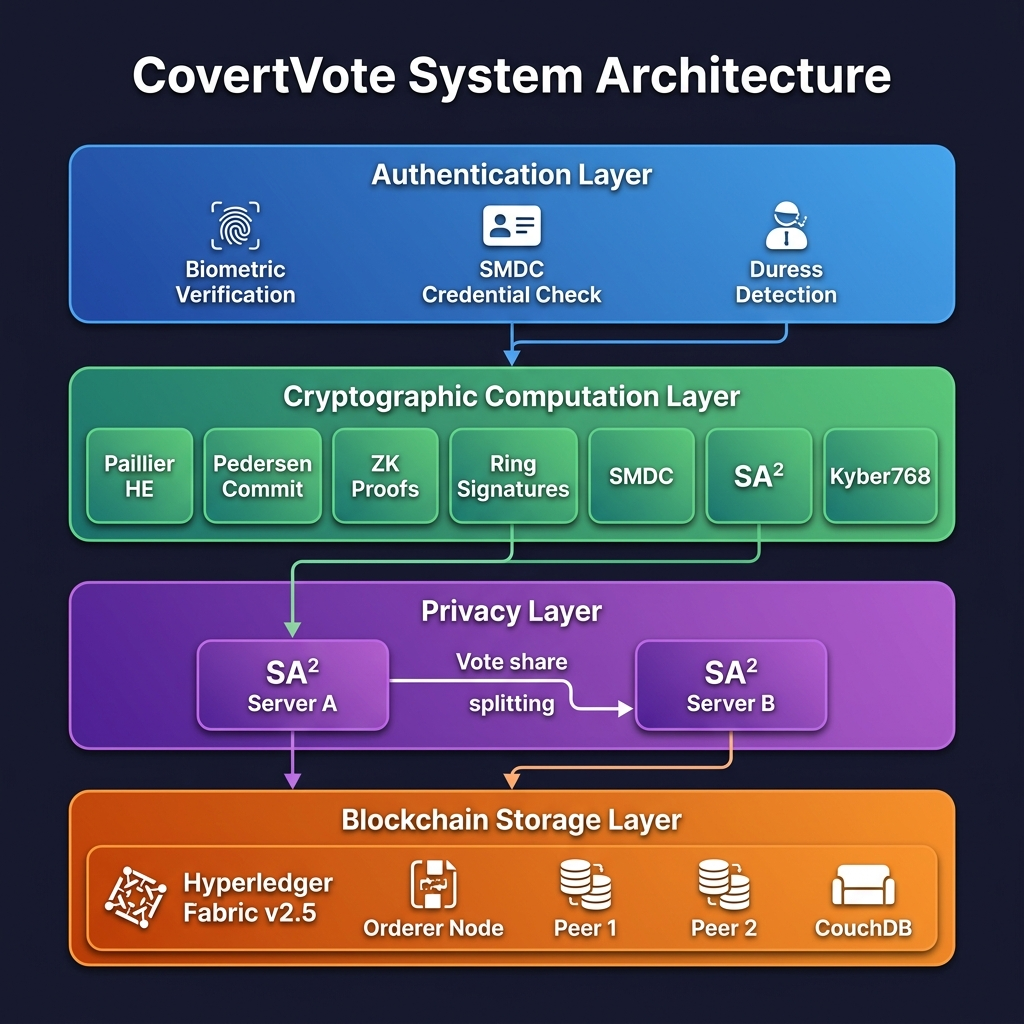
\includegraphics[width=0.85\textwidth]{Images/architecture.png}
\caption{Proposed System Architecture}
\label{fig:architecture}
\end{figure}

The framework operates under the following assumptions:

\begin{enumerate}
    \item The blockchain network consists of at least one ordering node and two peer nodes running Hyperledger Fabric v2.5 with Raft consensus.
    \item The two SA\textsuperscript{2} aggregation servers are operated by independent, non-colluding entities. The security guarantee holds as long as at least one server remains honest.
    \item Voters have access to a secure device for biometric authentication and vote submission.
    \item The election authority generates and distributes SMDC credentials to eligible voters before the election begins.
    \item The Paillier key pair is generated with a minimum of 2048-bit modulus for computational security.
    \item Each voter is assigned $k=5$ credential slots (1 real, 4 fake) for coercion resistance.
\end{enumerate}

\section{Notation}
\label{sec:notation}

Table~\ref{tab:notation} summarizes the mathematical symbols used throughout this chapter.

\begin{table}[H]
\centering
\caption{Mathematical Notation}
\label{tab:notation}
\small
\begin{tabular}{|c|p{10cm}|}
\hline
\textbf{Symbol} & \textbf{Meaning} \\
\hline
$p, q$ & Large primes for key generation \\
\hline
$n$ & RSA modulus $n = p \times q$ (Paillier) \\
\hline
$g$ & Generator; $g = n + 1$ for Paillier, subgroup generator for Pedersen \\
\hline
$h$ & Independent generator for Pedersen ($\log_g h$ unknown) \\
\hline
$\lambda$ & $\text{lcm}(p-1, q-1)$ (Paillier private key component) \\
\hline
$\mu$ & $L(g^\lambda \bmod n^2)^{-1} \bmod n$ (Paillier decryption parameter) \\
\hline
$L(x)$ & $L(x) = (x-1)/n$ (Paillier L-function) \\
\hline
$E(m)$ & Paillier encryption of message $m$: $g^m \cdot r^n \bmod n^2$ \\
\hline
$C$ & Pedersen commitment: $C = g^m \cdot h^r \bmod p$ \\
\hline
$r$ & Randomness for encryption or commitment \\
\hline
$w_i$ & Vote weight for candidate $i$; $w_i \in \{0, 1\}$, $\sum w_i = 1$ \\
\hline
$k$ & Number of SMDC credential slots (default $k = 5$) \\
\hline
$I$ & Key image for linkable ring signature: $I = H(\text{pk})^{\text{sk}}$ \\
\hline
$\sigma$ & Ring signature tuple $(I, c_0, r_0, r_1, \ldots, r_{n-1})$ \\
\hline
$\text{pk}_i, \text{sk}_i$ & Public/private key pair for ring member $i$ \\
\hline
$\mathcal{R}$ & Ring of public keys $\{\text{pk}_1, \ldots, \text{pk}_n\}$ with $|\mathcal{R}| = 100$ \\
\hline
$S_A, S_B$ & SA\textsuperscript{2} vote shares for Server A and Server B \\
\hline
$\text{mask}$ & Random masking value for SA\textsuperscript{2} share splitting \\
\hline
\end{tabular}
\end{table}

\section{Cryptographic Protocol Formulation}
\label{sec:crypto-formulation}

This section presents the mathematical formulation of all seven cryptographic protocols implemented in our framework. Each protocol provides a specific security guarantee, and their composition forms the complete voting pipeline.

\subsection{Paillier Homomorphic Encryption}
\label{subsec:paillier}

The Paillier cryptosystem~\cite{paillier1999} is an additively homomorphic public-key encryption scheme based on the Decisional Composite Residuosity Assumption (DCRA). It enables the computation of vote tallies directly on encrypted ballots without decryption.

\subsubsection{Key Generation}
\label{subsubsec:paillier-keygen}

The key generation process proceeds as follows:

\begin{enumerate}
    \item Select two large primes $p$ and $q$ of equal length ($\geq 1024$ bits each), ensuring $p \neq q$.
    \item Compute the RSA modulus:
    \begin{equation}
        n = p \times q
        \label{eq:paillier-n}
    \end{equation}
    \item Compute Carmichael's function:
    \begin{equation}
        \lambda = \text{lcm}(p-1, q-1)
        \label{eq:paillier-lambda}
    \end{equation}
    \item Set the generator $g = n + 1$ (standard choice that simplifies computation).
    \item Compute the decryption parameter:
    \begin{equation}
        \mu = L(g^\lambda \bmod n^2)^{-1} \bmod n
        \label{eq:paillier-mu}
    \end{equation}
    where $L(x) = \frac{x-1}{n}$.
\end{enumerate}

The public key is $(n, g, n^2)$ and the private key is $(\lambda, \mu, p, q)$.

\subsubsection{Encryption}
\label{subsubsec:paillier-enc}

To encrypt a plaintext message $m \in \mathbb{Z}_n$:
\begin{enumerate}
    \item Select a random $r \in \mathbb{Z}_n^*$ where $r > 0$.
    \item Compute the ciphertext:
    \begin{equation}
        c = g^m \cdot r^n \bmod n^2
        \label{eq:paillier-enc}
    \end{equation}
\end{enumerate}

\subsubsection{Decryption}
\label{subsubsec:paillier-dec}

To decrypt a ciphertext $c$:
\begin{equation}
    m = L(c^\lambda \bmod n^2) \cdot \mu \bmod n
    \label{eq:paillier-dec}
\end{equation}

\subsubsection{Homomorphic Properties}
\label{subsubsec:paillier-homo}

The Paillier cryptosystem supports the following homomorphic operations:

\textbf{Additive Homomorphism.} The product of two ciphertexts decrypts to the sum of their plaintexts:
\begin{equation}
    E(m_1) \cdot E(m_2) \bmod n^2 = E(m_1 + m_2)
    \label{eq:homo-add}
\end{equation}

This property is the foundation of the proposed framework's $O(n)$ tally. Given $n$ encrypted votes $\{E(v_1), E(v_2), \ldots, E(v_n)\}$ for a single candidate, the encrypted tally is:
\begin{equation}
    E\left(\sum_{i=1}^{n} v_i\right) = \prod_{i=1}^{n} E(v_i) \bmod n^2
    \label{eq:tally}
\end{equation}

\textbf{Scalar Multiplication.} A ciphertext raised to a scalar $k$ yields the encryption of $k \times m$:
\begin{equation}
    E(m)^k \bmod n^2 = E(k \cdot m)
    \label{eq:homo-scalar}
\end{equation}

\subsection{Pedersen Commitments}
\label{subsec:pedersen}

Pedersen commitments~\cite{pedersen1991} provide computationally hiding and perfectly binding commitments, serving as the foundation for zero-knowledge proofs in our framework.

\subsubsection{Parameter Generation}
\label{subsubsec:pedersen-params}

\begin{enumerate}
    \item Generate a safe prime $p = 2q + 1$ where $q$ is also prime.
    \item Find a generator $g$ of the subgroup of order $q$: select random $h \in \mathbb{Z}_p^*$ and compute $g = h^{(p-1)/q} \bmod p$ until $g \neq 1$.
    \item Derive an independent generator $h$ such that $\log_g h$ is unknown, using hash-to-group: $h = \text{SHA3}(g)^{(p-1)/q} \bmod p$.
\end{enumerate}

\subsubsection{Commitment}
\label{subsubsec:pedersen-commit}

To commit to a value $m \in \mathbb{Z}_q$ with randomness $r \in \mathbb{Z}_q$:
\begin{equation}
    C = g^m \cdot h^r \bmod p
    \label{eq:pedersen}
\end{equation}

\textbf{Security Properties:}
\begin{itemize}
    \item \textbf{Computationally Hiding}: Given $C$, no polynomial-time adversary can determine $m$ (under the Discrete Logarithm assumption).
    \item \textbf{Perfectly Binding}: There exists no $(m', r') \neq (m, r)$ such that $g^{m'} \cdot h^{r'} = g^m \cdot h^r$ (information-theoretically).
\end{itemize}

\textbf{Homomorphic Property:}
\begin{equation}
    C_1 \cdot C_2 = g^{m_1+m_2} \cdot h^{r_1+r_2} \bmod p = \text{Commit}(m_1 + m_2, r_1 + r_2)
    \label{eq:pedersen-homo}
\end{equation}

\subsection{Zero-Knowledge Proofs ($\Sigma$-Protocol)}
\label{subsec:zkp}

Our framework implements two zero-knowledge proofs using the Strong Fiat-Shamir transformation~\cite{bernhard2012}: a binary proof ($w \in \{0, 1\}$) and a sum proof ($\sum w_i = 1$).

\subsubsection{Binary Proof}
\label{subsubsec:binary-proof}

The binary proof demonstrates that a Pedersen commitment $C = g^w \cdot h^r$ contains either $w = 0$ or $w = 1$, without revealing which. This uses an OR-composition of two Schnorr-like proofs.

\textbf{Proof Generation} (for $w = 0$; the $w = 1$ case is symmetric):
\begin{enumerate}
    \item \textbf{Simulate} the $w = 1$ branch: choose random $d_1, r_1 \in \mathbb{Z}_q$ and compute:
    \begin{equation}
        A_1 = g \cdot h^{r_1} \cdot (C/g)^{-d_1} \bmod p
    \end{equation}
    \item \textbf{Real proof} for $w = 0$: choose random $r_0 \in \mathbb{Z}_q$ and compute:
    \begin{equation}
        A_0 = h^{r_0} \bmod p
    \end{equation}
    \item Compute the Strong Fiat-Shamir challenge:
    \begin{equation}
        c = H(\text{params} \| \text{nonce} \| \text{electionID} \| C \| A_0 \| A_1) \bmod q
        \label{eq:fiat-shamir}
    \end{equation}
    where $\text{params} = (p, q, g, h)$ are included per the Bernhard-Pereira-Warinschi recommendation.
    \item Compute $d_0 = c - d_1 \bmod q$ and $f_0 = r_0 + d_0 \cdot r \bmod q$.
\end{enumerate}

The proof is $\pi = (A_0, A_1, d_0, d_1, f_0, f_1, \text{nonce}, \text{electionID})$.

\textbf{Verification:}
\begin{enumerate}
    \item Check $d_0 + d_1 \equiv c \pmod{q}$
    \item Check $h^{f_0} \cdot C^{-d_0} \equiv A_0 \pmod{p}$
    \item Check $g \cdot h^{f_1} \cdot (C/g)^{-d_1} \equiv A_1 \pmod{p}$
\end{enumerate}

\subsubsection{Sum Proof}
\label{subsubsec:sum-proof}

The sum proof demonstrates that $\sum_{i=1}^{m} w_i = 1$ across all candidate commitments, ensuring each voter selects exactly one candidate.

Given commitments $\{C_1, \ldots, C_m\}$ with randomness $\{r_1, \ldots, r_m\}$:
\begin{enumerate}
    \item Compute the product: $\Pi = \prod_{i=1}^{m} C_i = g^{\sum w_i} \cdot h^{\sum r_i} \bmod p$
    \item Since $\sum w_i = 1$, we have $\Pi = g \cdot h^{R} \bmod p$ where $R = \sum r_i \bmod q$.
    \item Execute a Schnorr proof of knowledge of $R$: choose random $k$, compute $A = h^k$, challenge $c = H(\text{params} \| \Pi \| A \| g)$, response $s = k + c \cdot R \bmod q$.
\end{enumerate}

\textbf{Verification:} Recompute $A$ from $(s, c)$: check $h^s \cdot (\Pi/g)^{-c} \equiv A \pmod{p}$.

\subsection{Linkable Ring Signatures}
\label{subsec:ring-sig}

Our framework uses linkable ring signatures based on the Liu-Wei-Wong construction~\cite{liu2004} with a fixed ring size of $|\mathcal{R}| = 100$ members.

\subsubsection{Key Generation}
\label{subsubsec:ring-keygen}

Each voter generates a key pair:
\begin{equation}
    \text{sk} \xleftarrow{\$} \mathbb{Z}_q, \quad \text{pk} = g^{\text{sk}} \bmod p
    \label{eq:ring-keygen}
\end{equation}

\subsubsection{Signing}
\label{subsubsec:ring-sign}

Given message $M$, signer key $(\text{sk}_s, \text{pk}_s)$, ring $\mathcal{R} = \{\text{pk}_0, \ldots, \text{pk}_{n-1}\}$, and signer index $s$:

\begin{enumerate}
    \item Compute the key image (for double-vote detection):
    \begin{equation}
        I = H(\text{pk}_s)^{\text{sk}_s} \bmod p
        \label{eq:key-image}
    \end{equation}
    \item Choose random $\alpha \in \mathbb{Z}_q$ and compute:
    \begin{equation}
        L_s = g^\alpha \bmod p, \quad R_s = H(\text{pk}_s)^\alpha \bmod p
    \end{equation}
    \item Set $c_{s+1} = H(M \| L_s \| R_s)$.
    \item For each non-signer $i \neq s$ (in cyclic order), choose random $r_i$ and compute:
    \begin{equation}
        L_i = g^{r_i} \cdot \text{pk}_i^{c_i} \bmod p, \quad R_i = H(\text{pk}_i)^{r_i} \cdot I^{c_i} \bmod p
    \end{equation}
    \begin{equation}
        c_{i+1} = H(M \| L_i \| R_i)
    \end{equation}
    \item Close the ring: $r_s = \alpha - c_s \cdot \text{sk}_s \bmod q$.
\end{enumerate}

The signature is $\sigma = (I, c_0, r_0, r_1, \ldots, r_{n-1})$.

\subsubsection{Verification and Linkability}
\label{subsubsec:ring-verify}

Verification reconstructs all $(L_i, R_i)$ pairs and checks that the ring closes: the final computed challenge equals $c_0$. Linkability is achieved through key images: two signatures from the same signer produce identical $I$ values, enabling double-vote detection via $I_1 \stackrel{?}{=} I_2$.
% Chapter 3 Part B - Continuation
% This file is merged with chapter3a.tex into chapter3.tex

\subsection{SMDC: Self-Masking Deniable Credentials}
\label{subsec:smdc}

SMDC is a novel coercion resistance mechanism designed for our framework. Each voter receives $k = 5$ credential slots, of which exactly one is real (weight $= 1$) and the remaining four are fake (weight $= 0$). The real slot index is derived deterministically via HMAC and is never stored, ensuring only the legitimate voter can identify it.

\subsubsection{Credential Generation}
\label{subsubsec:smdc-gen}

For voter with identifier $\text{vid}$ in election $\text{eid}$:

\begin{enumerate}
    \item \textbf{Derive real index} (deterministic, re-derivable):
    \begin{equation}
        \text{idx}_{\text{real}} = \text{HMAC-SHA256}(\text{eid}, \text{``smdc-real-index:''} \| \text{vid} \| \text{eid}) \bmod k
        \label{eq:smdc-index}
    \end{equation}
    
    \item \textbf{Create $k$ slots}: For each slot $i \in \{0, \ldots, k-1\}$:
    \begin{equation}
        w_i = \begin{cases} 1 & \text{if } i = \text{idx}_{\text{real}} \\ 0 & \text{otherwise} \end{cases}
    \end{equation}
    
    \item \textbf{Commit}: Generate Pedersen commitment for each slot:
    \begin{equation}
        C_i = g^{w_i} \cdot h^{r_i} \bmod p, \quad r_i \xleftarrow{\$} \mathbb{Z}_q
        \label{eq:smdc-commit}
    \end{equation}
    
    \item \textbf{Prove binary}: For each $C_i$, generate a ZK proof $\pi_i^{\text{bin}}$ that $w_i \in \{0, 1\}$.
    
    \item \textbf{Prove sum}: Generate proof $\pi^{\text{sum}}$ that $\sum_{i=0}^{k-1} w_i = 1$.
\end{enumerate}

The credential is $\text{Cred} = (\text{vid}, k, \{(C_i, \pi_i^{\text{bin}})\}_{i=0}^{k-1}, \pi^{\text{sum}})$.

\subsubsection{Coercion Resistance Property}
\label{subsubsec:smdc-coercion}

Under coercion, the voter presents a \emph{fake} slot $j \neq \text{idx}_{\text{real}}$. The coercer observes:
\begin{itemize}
    \item A valid Pedersen commitment $C_j = g^0 \cdot h^{r_j} = h^{r_j}$
    \item A valid binary proof $\pi_j^{\text{bin}}$ (proving $w_j \in \{0, 1\}$, without revealing $w_j = 0$)
    \item A valid sum proof $\pi^{\text{sum}}$ (proving exactly one slot has $w = 1$)
\end{itemize}

Due to Pedersen's \textbf{computational hiding} property, the coercer cannot determine whether $C_j$ commits to 0 or 1. The vote cast with a fake credential is silently discarded during tally (it contributes $w = 0$ to the homomorphic sum), while the voter's receipt appears identical to a real vote receipt. Figure~\ref{fig:smdc} illustrates this mechanism.

\begin{figure}[H]
\centering
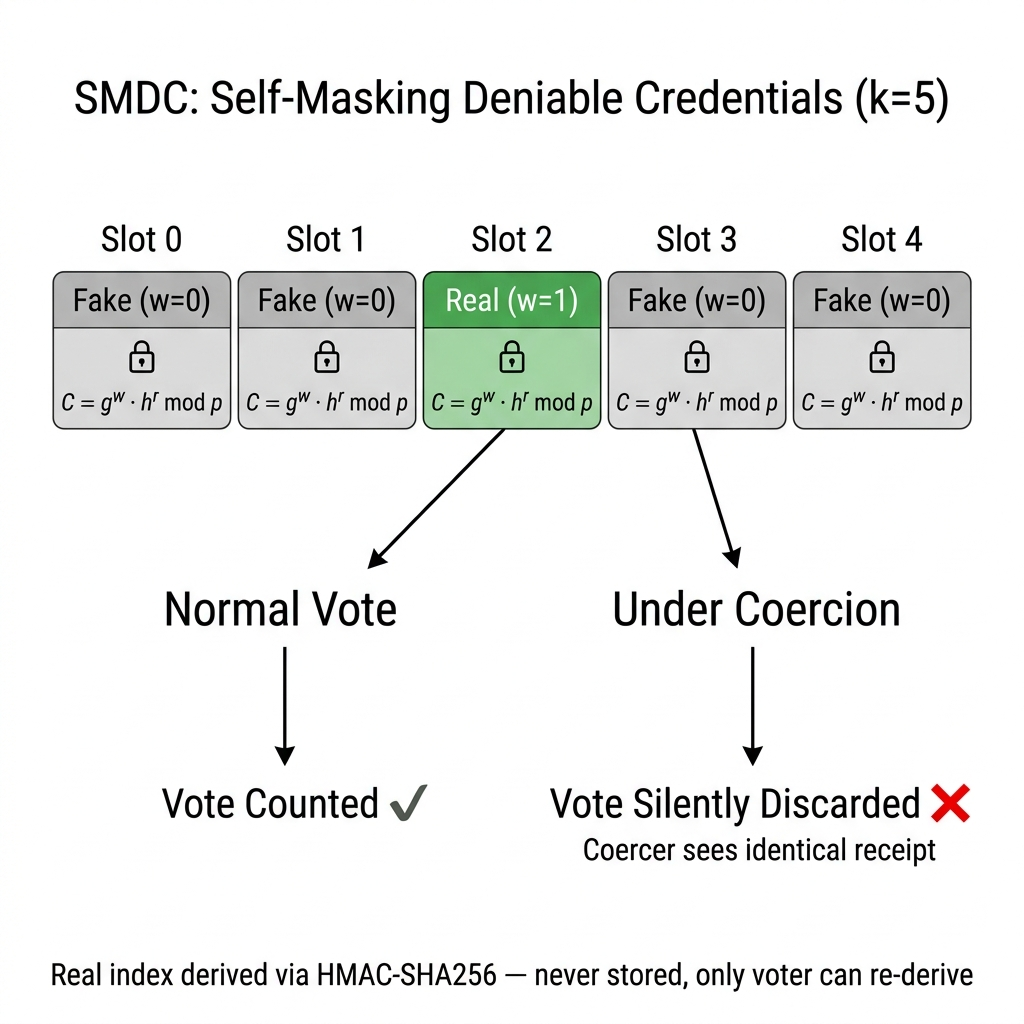
\includegraphics[width=0.75\textwidth]{Images/smdc.png}
\caption{SMDC Deniable Credential Structure ($k=5$)}
\label{fig:smdc}
\end{figure}

\subsubsection{Credential Verification}
\label{subsubsec:smdc-verify}

The election system verifies credentials without learning the real index:
\begin{enumerate}
    \item Verify all $k$ binary proofs: $\forall i: \text{VerifyBinary}(C_i, \pi_i^{\text{bin}}) = \text{true}$
    \item Verify the sum proof: $\text{VerifySumOne}(\{C_i\}, \pi^{\text{sum}}) = \text{true}$
\end{enumerate}

\subsection{SA\textsuperscript{2}: Samplable Anonymous Aggregation}
\label{subsec:sa2}

Our framework adapts Apple's Samplable Anonymous Aggregation (SA\textsuperscript{2}) protocol~\cite{sa2_apple}, building on the foundational work by Bonawitz et al.~\cite{bonawitz2017} on practical secure aggregation for privacy-preserving machine learning. Originally designed for federated data analysis, the SA\textsuperscript{2} protocol is adapted here for voting to provide a two-server privacy model for vote aggregation.

\subsubsection{Vote Splitting}
\label{subsubsec:sa2-split}

Given an encrypted vote $E(v)$ for voter $u$:

\begin{enumerate}
    \item Generate a random mask: $\text{mask} \xleftarrow{\$} \mathbb{Z}_{n/100}$
    \item Compute Share A (for Server A):
    \begin{equation}
        S_A = E(v) \cdot E(\text{mask}) = E(v + \text{mask}) \bmod n^2
        \label{eq:sa2-share-a}
    \end{equation}
    \item Compute Share B (for Server B):
    \begin{equation}
        S_B = E(-\text{mask}) = E(n - \text{mask}) \bmod n^2
        \label{eq:sa2-share-b}
    \end{equation}
\end{enumerate}

\subsubsection{Reconstruction}
\label{subsubsec:sa2-reconstruct}

Due to Paillier's additive homomorphism:
\begin{equation}
    S_A \cdot S_B = E(v + \text{mask}) \cdot E(-\text{mask}) = E(v) \bmod n^2
    \label{eq:sa2-reconstruct}
\end{equation}

\textbf{Security Guarantee:} As long as at least one of the two servers remains honest and does not share its received share with the other server, no individual vote $v$ can be reconstructed. Server A sees only $E(v + \text{mask})$ and Server B sees only $E(-\text{mask})$; neither can derive $E(v)$ alone.

\subsection{Kyber768 Post-Quantum Hybrid Encryption}
\label{subsec:kyber}

To protect against future quantum computer attacks, Our framework implements a hybrid encryption scheme combining classical Paillier encryption with NIST-standardized Kyber768 (ML-KEM)~\cite{nist_kyber} key encapsulation.

\subsubsection{Hybrid Encryption Scheme}
\label{subsubsec:hybrid}

The hybrid scheme operates as follows:
\begin{enumerate}
    \item \textbf{Kyber Key Generation}: Generate a Kyber768 key pair $(\text{pk}_{\text{ky}}, \text{sk}_{\text{ky}})$ providing NIST Level 3 security (equivalent to AES-192).
    \item \textbf{Paillier Encryption}: Encrypt the vote with Paillier to preserve homomorphic properties:
    \begin{equation}
        E(v) = g^v \cdot r^n \bmod n^2
    \end{equation}
    \item \textbf{Encapsulation}: Generate a shared secret $K$ and ciphertext $\text{ct}_{\text{ky}}$:
    \begin{equation}
        (K, \text{ct}_{\text{ky}}) = \text{Kyber.Encapsulate}(\text{pk}_{\text{ky}})
    \end{equation}
    \item \textbf{Key Derivation}: Derive an authentication key: $K_{\text{auth}} = \text{SHA256}(K \| \text{salt})$.
    \item \textbf{MAC Authentication}: Compute HMAC-SHA256 over the Paillier ciphertext:
    \begin{equation}
        \text{MAC} = \text{HMAC-SHA256}(K_{\text{auth}}, E(v))
    \end{equation}
    \item \textbf{Transmission}: Send $(\text{ct}_{\text{ky}}, E(v), \text{salt}, \text{MAC})$.
\end{enumerate}

This hybrid construction ensures dual-layer protection: the Paillier ciphertext $E(v)$ provides semantic security under DCRA and preserves homomorphic properties for tallying, while the Kyber768 layer provides a post-quantum integrity binding via the MAC. An adversary must compromise \emph{both} layers to tamper with votes undetected. The generic message encryption functions additionally use AES-256-GCM~\cite{nist_gcm} for symmetric encryption of non-homomorphic data.

\subsection{Threshold Paillier Decryption}
\label{subsec:threshold}

To prevent any single entity from decrypting election results, Our framework implements the Damg\aa rd-Jurik-Nielsen (DJN)~\cite{damgard2010} threshold decryption scheme with Shamir's Secret Sharing.

\subsubsection{Key Distribution}
\label{subsubsec:threshold-dist}

The private key $\lambda$ is split into $n$ shares using $(t, n)$-Shamir Secret Sharing~\cite{shamir1979}, where at least $t$ parties must cooperate for decryption. Each party $i$ receives share $\lambda_i$.

\subsubsection{Partial Decryption}
\label{subsubsec:threshold-partial}

Each party $i$ computes a partial decryption with a ZK proof of correctness:
\begin{equation}
    d_i = c^{\lambda_i} \bmod n^2
    \label{eq:partial-dec}
\end{equation}

\subsubsection{Combination}
\label{subsubsec:threshold-combine}

Given $t$ valid partial decryptions, Lagrange interpolation reconstructs the plaintext:
\begin{equation}
    m = L\left(\prod_{i \in S} d_i^{\delta_i} \bmod n^2\right) \cdot \mu \bmod n
    \label{eq:threshold-combine}
\end{equation}
where $\delta_i = \prod_{j \in S, j \neq i} \frac{j}{j - i}$ are Lagrange coefficients and $S$ is the set of participating parties.

\section{Vote Casting Pipeline}
\label{sec:pipeline}

Figure~\ref{fig:pipeline} illustrates the four-phase pipeline, and Algorithm~\ref{alg:pipeline} presents the formal pseudocode.

\begin{figure}[H]
\centering
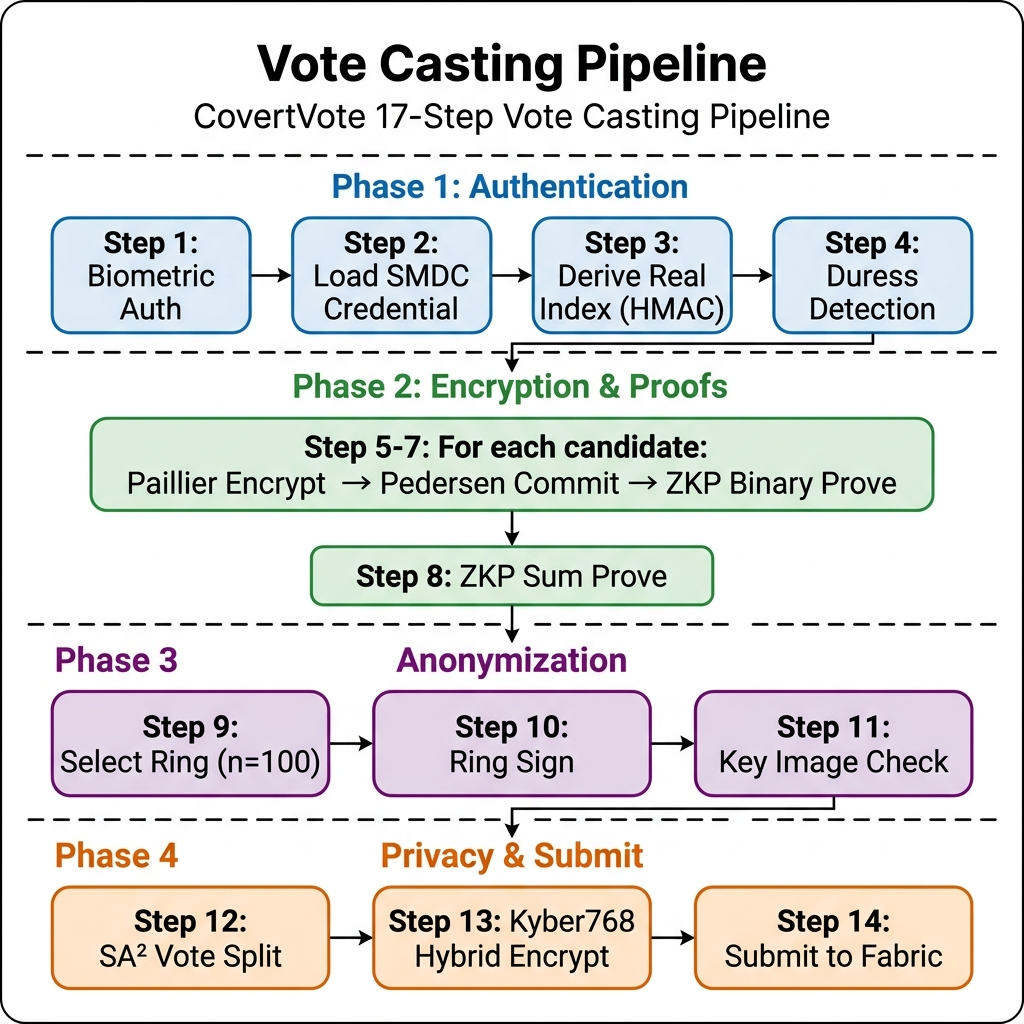
\includegraphics[width=0.8\textwidth]{Images/pipeline.png}
\caption{Proposed Vote Casting Pipeline}
\label{fig:pipeline}
\end{figure}

\begin{algorithm}[H]
\caption{Proposed 17-Step Vote Casting Pipeline}
\label{alg:pipeline}
\begin{algorithmic}[1]
\Require Voter ID $\text{vid}$, candidate selection $j$, credentials, keys
\Ensure Encrypted, signed, split vote record on blockchain

\State \textbf{// Phase 1: Authentication \& Credential}
\State Authenticate voter via biometric verification
\State Retrieve SMDC credential $\text{Cred}$
\State Derive real index: $\text{idx} \gets \text{HMAC}(\text{eid}, \text{vid})  \bmod k$
\State Check duress signals via behavioral detection

\State \textbf{// Phase 2: Vote Encryption}
\For{each candidate $i \in \{1, \ldots, m\}$}
    \State Set $w_i = 1$ if $i = j$, else $w_i = 0$
    \State Encrypt: $E_i \gets \text{Paillier.Encrypt}(w_i)$
    \State Commit: $C_i \gets g^{w_i} \cdot h^{r_i} \bmod p$
    \State Prove binary: $\pi_i^{\text{bin}} \gets \text{ProveBinary}(w_i, r_i, C_i)$
\EndFor
\State Prove sum: $\pi^{\text{sum}} \gets \text{ProveSumOne}(\{C_i\})$

\State \textbf{// Phase 3: Anonymization}
\State Select ring $\mathcal{R}$ of size 100 from voter pool
\State Sign ballot: $\sigma \gets \text{RingSign}(\text{ballot}, \text{sk}, \mathcal{R})$
\State Check key image $I$ against used images (double-vote detection)

\State \textbf{// Phase 4: Privacy \& Submission}
\State Split vote via SA\textsuperscript{2}: $(S_A, S_B) \gets \text{SplitVote}(E_i)$
\State Apply Kyber768 hybrid encryption to shares
\State Submit to Hyperledger Fabric via Gateway SDK
\end{algorithmic}
\end{algorithm}

\section{Blockchain Integration}
\label{sec:blockchain-integration}

Our framework uses Hyperledger Fabric v2.5 as its blockchain infrastructure. The deployment consists of:

\begin{itemize}
    \item \textbf{1 Raft Orderer Node}: Provides transaction ordering with crash fault tolerance.
    \item \textbf{2 Peer Nodes}: Maintain the distributed ledger and execute chaincode.
    \item \textbf{1 Certificate Authority}: Issues MSP identities for network participants.
\end{itemize}

The chaincode (smart contract), written in Go, implements the following functions:

\begin{itemize}
    \item \texttt{CreateElection}: Initializes an election with metadata and candidate list.
    \item \texttt{CastVote}: Records an encrypted vote with ZK proofs and ring signature.
    \item \texttt{GetElection}: Queries election state from the world state database.
    \item \texttt{TallyVotes}: Performs homomorphic aggregation of encrypted votes.
\end{itemize}

Application-level communication uses the Fabric Gateway SDK (v1.10.1) with gRPC/TLS connections, providing authenticated, encrypted communication between the voting application and peer nodes.

\section{Engineering and Societal Considerations}
\label{sec:engineering}

\subsection{Societal Impact}
The proposed framework addresses voter coercion, a problem particularly prevalent in developing nations where family voting, vote buying, and employer pressure undermine democratic processes. The SMDC mechanism provides mathematical guarantees of coercion resistance, potentially improving electoral integrity for billions of voters worldwide.

\subsection{Sustainability}
Unlike proof-of-work blockchain systems, Hyperledger Fabric uses Raft consensus, which requires minimal energy. The environmental footprint of the proposed framework is comparable to a standard web application.

\subsection{Accessibility}
The system is designed for remote voting, improving accessibility for voters with mobility challenges, those in remote areas, or overseas citizens.

\subsection{Ethical Considerations}
The deniable credential mechanism raises ethical questions about vote accountability. While coercion resistance protects voters, it also makes it impossible to prove how any individual voted, which is by design a fundamental requirement of democratic elections.

\section{Security Analysis}
\label{sec:security-analysis}

This section presents the formal security properties of the proposed framework. Each theorem corresponds to a specific security guarantee provided by the cryptographic protocols described in Sections~\ref{sec:crypto-formulation}--\ref{sec:pipeline}.

\subsection{Formal Security Theorems}
\label{subsec:security-theorems}

\textbf{Theorem 1 (Ballot Privacy).} \textit{Under the Decisional Composite Residuosity Assumption (DCRA), no probabilistic polynomial-time adversary can distinguish $E(v_i)$ from $E(v_j)$ for any two valid vote values $v_i, v_j \in \{0, 1\}$.}

\textit{Proof Sketch.} The semantic security of the Paillier cryptosystem guarantees that $E(0)$ and $E(1)$ are computationally indistinguishable. Given ciphertext $c = g^m \cdot r^n \bmod n^2$ with random $r \xleftarrow{\$} \mathbb{Z}_n^*$, distinguishing $m = 0$ from $m = 1$ requires solving the DCRA problem, which is reducible to factoring $n = p \cdot q$ with $|p| = |q| = 1024$ bits. Our implementation uses 2048-bit modulus, providing $\geq 112$-bit security. \hfill $\square$

\textbf{Theorem 2 (Vote Validity).} \textit{The zero-knowledge $\Sigma$-proofs (binary + sum) ensure that every counted vote satisfies $w_i \in \{0, 1\}$ for each candidate and $\sum_{i=1}^{m} w_i = 1$, with soundness error $\leq 2^{-256}$.}

\textit{Proof Sketch.} The binary proof uses an OR-composition of two Schnorr proofs, achieving special soundness: an extractor can recover the witness from two accepting transcripts with distinct challenges. The Strong Fiat-Shamir transformation with domain separation (including public parameters in the hash per Bernhard-Pereira-Warinschi~\cite{bernhard2012}) ensures non-interactive soundness in the random oracle model. The sum proof is a standard Schnorr proof of knowledge of the discrete log $R = \sum r_i$ satisfying $\Pi/g = h^R$. With SHA-256 producing 256-bit challenges, the soundness error is bounded by $2^{-256}$. \hfill $\square$

\textbf{Theorem 3 (Voter Anonymity).} \textit{Given a valid ring signature $\sigma = (I, c_0, r_0, \ldots, r_{n-1})$ with ring size $|\mathcal{R}| = 100$, no adversary can identify the actual signer with probability greater than $1/|\mathcal{R}| = 0.01$, under the Decisional Diffie-Hellman (DDH) assumption.}

\textit{Proof Sketch.} The Liu-Wei-Wong linkable ring signature scheme~\cite{liu2004} achieves signer ambiguity: for each non-signer $i$, the values $(c_i, r_i)$ are sampled uniformly at random during signing, making them statistically indistinguishable from the signer's values $(c_s, r_s = \alpha - c_s \cdot \text{sk}_s)$ under DDH. The key image $I = H(\text{pk}_s)^{\text{sk}_s}$ enables linkability (double-vote detection) without revealing the signer's identity, as computing $\text{sk}_s$ from $I$ requires solving the discrete log problem. \hfill $\square$

\textbf{Theorem 4 (Coercion Resistance).} \textit{Given SMDC credentials with $k = 5$ slots, a coercer observing a voter's credential usage cannot distinguish whether the presented slot $j$ is real ($w_j = 1$) or fake ($w_j = 0$), under the Computational Hiding property of Pedersen commitments.}

\textit{Proof Sketch.} Each slot $i$ has commitment $C_i = g^{w_i} \cdot h^{r_i} \bmod p$ with independent randomness $r_i$. By Pedersen's computational hiding property (under DLog), distinguishing $C_i = g^0 \cdot h^{r_i}$ from $C_i = g^1 \cdot h^{r_i}$ requires computing $\log_g h$, which is infeasible. The accompanying ZK proofs $\pi_i^{\text{bin}}$ are zero-knowledge (simulator exists), so they leak no information about $w_i$. The real index $\text{idx}_{\text{real}}$ is derived via HMAC-SHA256 and never stored, making it re-derivable only by the legitimate voter who knows $\text{vid}$ and $\text{eid}$. A coerced vote contributes $w = 0$ to the homomorphic tally, silently discarded without any observable difference. \hfill $\square$

\textbf{Theorem 5 (Aggregation Privacy).} \textit{Under the SA\textsuperscript{2} two-server model, no individual vote $v$ can be reconstructed as long as at least one of the two servers remains honest.}

\textit{Proof Sketch.} Server A receives $S_A = E(v + \text{mask})$ and Server B receives $S_B = E(-\text{mask})$, where $\text{mask} \xleftarrow{\$} \mathbb{Z}_{n/100}$. Under Paillier's semantic security, Server A cannot distinguish $S_A$ from a random element of $\mathbb{Z}_{n^2}^*$, and Server B's share $S_B$ is independent of $v$. Reconstruction requires $S_A \cdot S_B = E(v)$, which is possible only when both shares are combined. A corrupted single server gains no information about $v$ beyond what is implied by the final tally. \hfill $\square$

\textbf{Theorem 6 (Post-Quantum Encryption Layer).} \textit{The Kyber768 hybrid encryption provides a post-quantum integrity and confidentiality binding for vote ciphertexts during transit and storage. An adversary must break both the Paillier DCRA assumption and the Module-LWE assumption underlying Kyber768 (NIST Level 3, $\geq$ 192-bit classical security) to tamper with or forge vote records.}

\textit{Proof Sketch.} The hybrid scheme binds a Kyber768 KEM-derived key to each Paillier ciphertext via HMAC-SHA256 authentication. An adversary attempting to tamper with $E(v)$ must forge a valid MAC, which requires knowledge of the Kyber shared secret $K$. Computing $K$ from the KEM ciphertext requires solving Module-LWE, which is believed to be quantum-resistant per NIST's standardization of ML-KEM-768 (FIPS 203, August 2024). Generic message encryption additionally uses AES-256-GCM for authenticated symmetric encryption. Note that the homomorphic tallying operates on Paillier ciphertexts, which remain classically secure under DCRA. Similarly, the linkable ring signatures rely on the discrete logarithm assumption. Full post-quantum migration of these components (via lattice-based alternatives) is identified as future work in Chapter~\ref{ch:conclusion}. \hfill $\square$

\subsection{Duress Detection}
\label{subsec:duress-detection}

Our framework implements a behavioral duress detection mechanism that complements the SMDC credential system. Algorithm~\ref{alg:duress} presents the detection procedure.

\begin{algorithm}[H]
\caption{Behavioral Duress Detection}
\label{alg:duress}
\begin{algorithmic}[1]
\Require Biometric signals $\mathcal{B} = \{\text{blink\_count}, \text{head\_tilt}, \text{long\_press}, \text{time\_delay}, \text{voice\_cmd}\}$
\Require HMAC key $K_{\text{duress}}$, threshold $\theta$
\Ensure \textbf{true} if voter is under duress, \textbf{false} otherwise

\State Compute feature vector: $\mathbf{f} \gets \text{Normalize}(\mathcal{B})$
\State Compute duress hash: $h \gets \text{HMAC-SHA256}(K_{\text{duress}}, \mathbf{f})$
\State Extract score: $s \gets h[0:4] / 2^{32}$ \Comment{Normalize to $[0,1]$}
\If{$s > \theta$ \textbf{or} any signal exceeds critical bound}
    \State \textbf{return true} \Comment{Silently switch to fake credential}
\Else
    \State \textbf{return false}
\EndIf
\end{algorithmic}
\end{algorithm}

When duress is detected, the system silently substitutes the voter's real credential slot with a fake slot. The resulting vote is encrypted, signed, and submitted identically to a legitimate vote, but contributes $w = 0$ to the final tally. The voter receives an identical-looking receipt, ensuring the coercer cannot detect the substitution.

\section{Conclusion}
\label{sec:meth-conclusion}

This chapter presented the complete system design of the proposed framework, including the mathematical formulation of all seven cryptographic protocols, the 17-step vote casting pipeline, and the blockchain integration architecture. Six formal security theorems were stated with proof sketches, demonstrating that The proposed framework provides ballot privacy (Theorem 1), vote validity (Theorem 2), voter anonymity (Theorem 3), coercion resistance (Theorem 4), aggregation privacy (Theorem 5), and post-quantum security (Theorem 6). The key innovations are the SMDC coercion resistance mechanism with $k = 5$ deniable credential slots, the adaptation of SA\textsuperscript{2} for voting privacy, the behavioral duress detection system, and the Kyber768 hybrid encryption for post-quantum security. The next chapter presents the implementation details and comprehensive performance evaluation of the system.
